\documentclass[10pt]{article}
\usepackage[paperwidth=13cm, paperheight=23cm, margin=1cm]{geometry}
% Usuń numerację stron.
\pagestyle{empty}

\usepackage{tikz}
% Import do ustalania końcówek strzałek.
\usetikzlibrary{arrows.meta}

% Zmniejsz interlinię.
\linespread{0.9}

% Importy do białych konturów napisów.
\usepackage[T1]{fontenc}
\usepackage{pslatex}
\usepackage{contour}
\usepackage{color}
\contourlength{1pt} % Grubość konturu
\contournumber{50}  % Liczba powtórzeń

% Ustaw czcionkę bezszeryfową.
\renewcommand{\familydefault}{\sfdefault}

\begin{document}
\begin{figure}[p]
\centering
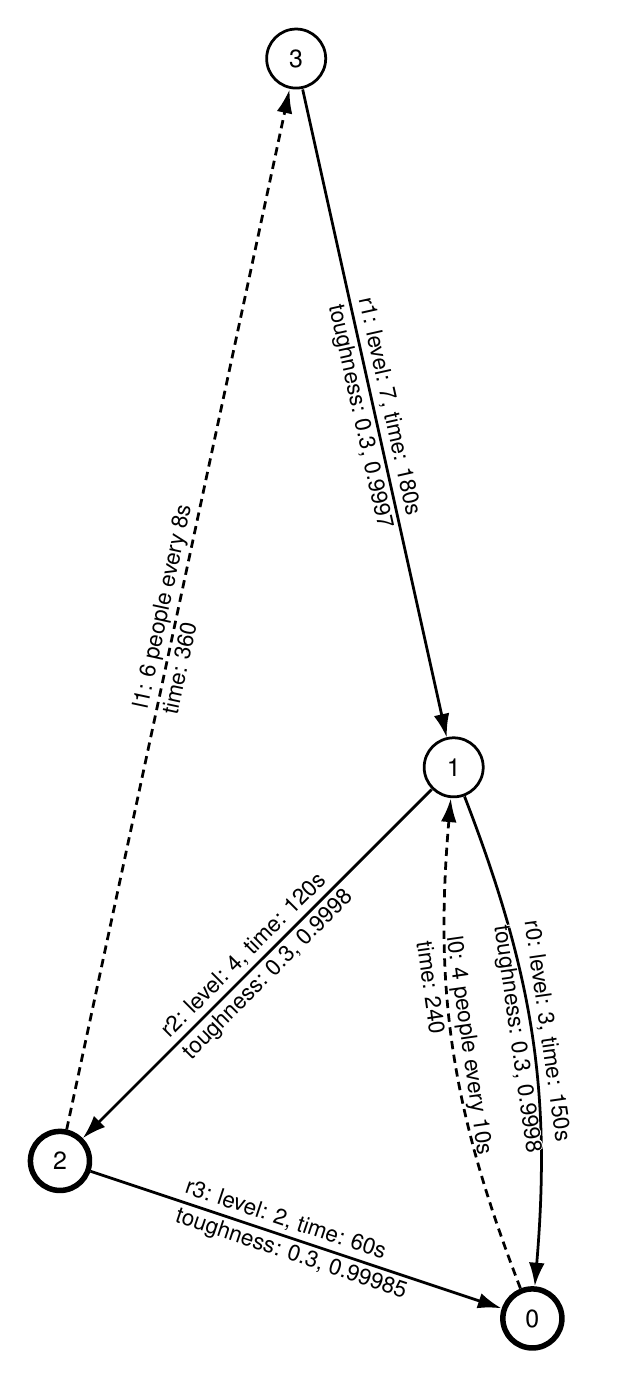
\begin{tikzpicture}[scale=100]
    \tikzset{
        % Style węzłów i krawędzi.
        wezel grafu/.style={circle,draw,minimum size=0.75cm,inner sep=0,line width=0.35mm},
        krawedz grafu/.style={-{Latex[length=3mm, width=2mm]},sloped,centered,line width=0.35mm,font=\small}
    }
    % Węzły:
    \node[wezel grafu,line width=0.7mm] (0) at (7/100, 1/100) {0};
    \node[wezel grafu] (1) at (6/100, 8/100) {1};
    \node[wezel grafu,line width=0.7mm] (2) at (1/100, 3/100) {2};
    \node[wezel grafu] (3) at (4/100, 17/100) {3};
    % Krawedzie:
    \path[draw]
    (0) edge[krawedz grafu, bend left=13, densely dashed] node {
        \begin{tabular}{l}
            \contour{white}{l0: 4 people every 10s} \\
            \contour{white}{time: 240}
        \end{tabular}
    } (1)
    (1) edge[krawedz grafu, bend left=13] node {
        \begin{tabular}{l}
            \contour{white}{r0: level: 3, time: 150s} \\
            \contour{white}{toughness: 0.3, 0.9998}
        \end{tabular}
    } (0)
    (2) edge[krawedz grafu] node {
        \begin{tabular}{l}
            \contour{white}{r3: level: 2, time: 60s} \\
            \contour{white}{toughness: 0.3, 0.99985}
        \end{tabular}
    } (0)
    (1) edge[krawedz grafu] node {
        \begin{tabular}{l}
            \contour{white}{r2: level: 4, time: 120s} \\
            \contour{white}{toughness: 0.3, 0.9998}
        \end{tabular}
    } (2)
    (3) edge[krawedz grafu] node {
        \begin{tabular}{l}
            \contour{white}{r1: level: 7, time: 180s} \\
            \contour{white}{toughness: 0.3, 0.9997}
        \end{tabular}
    } (1)
    (2) edge[krawedz grafu, densely dashed] node {
        \begin{tabular}{l}
            \contour{white}{l1: 6 people every 8s} \\
            \contour{white}{time: 360}
        \end{tabular}
    } (3)
    ;
\end{tikzpicture}

\end{figure}
\end{document}
